\documentclass{article}

\usepackage{geometry}
\usepackage{xeCJK}
\usepackage{amsmath}
\usepackage{tikz}
\usepackage{pgfplots}
% figure[H] float
\usepackage{float}
\usepackage{amssymb}
\usepackage{hyperref}
\usepackage{setspace}
% 字体底部样式:下划线、波浪线等
\usepackage{ulem}
% 修改公式编号
\usepackage{chngcntr}

% make cdot thicker,比 cdot 更粗的圆点
\makeatletter
\newcommand*\bigcdot{\mathpalette\bigcdot@{.5}}
\newcommand*\bigcdot@[2]{\mathbin{\vcenter{\hbox{\scalebox{#2}{$\m@th#1\bullet$}}}}}
\makeatother

% 设置行间距 1.5 倍
\renewcommand{\baselinestretch}{1.5}

% 设置页大小和页边距,或者scale=0.8
\geometry{a4paper,left=3.18cm,right=3.18cm,top=2.54cm,bottom=2.54cm}
% 兼容
\pgfplotsset{compat=1.16}
% 中文默认没有斜体和粗体格式,开启伪斜体和指定黑体;
\setCJKmainfont[AutoFakeSlant, BoldFont=SimHei]{SimSun}
\usetikzlibrary{positioning}
% area of hatch,面积阴影部分
\usetikzlibrary{patterns}
% 箭头类型
\usetikzlibrary{arrows.meta}

\hypersetup{
    colorlinks,
    citecolor=black,
    filecolor=black,
    linkcolor=black,
    urlcolor=black
}
% 定义amsmath arccot
\DeclareMathOperator{\arccot}{arccot}
% 每个章节后,重置公式编号
\counterwithin*{equation}{section}

% 修改公式标签引用颜色
\def\eqref#1{{\color{blue}\hypersetup{linkcolor=blue} (\ref{#1}) }}
% 修改图片标签引用的颜色
\def\figureref#1{{\color{blue}\hypersetup{linkcolor=blue} (\ref{#1}) }}

\begin{document}
  \tableofcontents
  \newpage

  \section{微分中值定理}
    \paragraph{}
本章将应用导数来研究函数以及曲线的某些形态,并利用这些知识解决一些实际问题。为此,先介绍微分学的几个中值定理,它们是导数应用的理论基础。

\subsection{罗尔定理(Rolle's theorem)}
\paragraph{}
\textbf{费马引理\;}设函数$f(x)$在点$x_0$的某邻域$U(x_0)$内有定义,并且在$x_0$处可导,如果对任意的$x\in U(x_0)$,有
\begin{equation}
  f(x) \leq f(x_0) \;(\text{或} f(x) \geq f(x_0)),
\end{equation}
那么$f'(x_0) = 0$。

\begin{figure}[H]
  \centering
    \input{figure/Fermat‘s_theorem}
    \label{Fermat‘s_theorem}
    \caption{费马引理}
\end{figure}

\paragraph{}
通常称导数等于零的点为函数的\uwave{驻点}(或\uwave{稳定点},\uwave{临界点})。

\paragraph{}
\textbf{罗尔定理\;}如果函数$f(x)$满足
\begin{enumerate}
  \item 在闭区间$[a,b]$上连续;
  \item 在开区间$(a,b)$内可导;
  \item 在区间端点处的函数值相等,即$f(a)=f(b)$,
\end{enumerate}
那么在$(a,b)$内至少有一点$\xi(a < \xi < b)$,使得$f'(\xi) = 0$。

\subsection{拉格朗日中值定理(Lagrange's mean value theorem)}
\subsubsection{定理}
\paragraph{}
罗尔定理中$f(a)=f(b)$这个条件是相当特殊的,它使罗尔定理的应用受到限制。如果把该条件取消,但仍保留其余两个条件,并相应的改变结论,那么得到微分学中十分重要的拉格朗日中值定理。

\paragraph{}
\textbf{拉格朗日中值定理\;}如果函数$f(x)$满足
\begin{enumerate}
  \item 在闭区间$[a,b]$上连续;
  \item 在开区间$(a,b)$内可导,
\end{enumerate}
那么在$(a,b)$内至少有一点$\xi(a < \xi < b)$,使等式
\begin{equation}
  f(b) - f(a) = f'(\xi)(b-a)
\end{equation}
成立。

\begin{figure}[H]
  \centering
    \input{figure/Lagrange‘s_mean_value_theorem}
    \caption{拉格朗日中值定理}
    \label{Lagrange‘s mean value theorem}
\end{figure}

\paragraph{}
从图\figureref{Lagrange‘s mean value theorem}中看出,在罗尔定理中,由于$f(a)=f(b)$,弦$AB$是平行于$x$轴的,因此点$C$处的切线实际上也平行于弦$AB$。由此可见,罗尔定理是拉格朗日中值定理的特殊情形。

\subsubsection{证明}
\paragraph{}
\textbf{证明前的准备\;}使用罗尔定理来证明拉格朗日中值定理。

\paragraph{}
在拉格朗日中值定理中,函数$f(x)$不一定具备$f(a)=f(b)$这个条件,为此我们设想构造一个与$f(x)$有密切联系的函数$\varphi(x)$(称为\uwave{辅助函数}),使$\varphi(x)$满足条件$\varphi(a) = \varphi(b)$。然后应用罗尔定理。

\paragraph{}
从图\figureref{Lagrange‘s mean value theorem}中看到,有向线段$NM$的值是与$x$有关联的函数,把它表示为$\varphi(x)$,它与$f(x)$有密切的联系,且当$x=a$及$x=b$时,点$M$与点$N$重合,即有$\varphi(a)=\varphi(b)=0$。为求得函数$\varphi(x)$的表达式,设直线$AB$的方程为$y=L(x)$,则

\begin{equation*}
  L(x) = f(a) + \frac{f(b) - f(a)}{b - a}(x-a)
\end{equation*}

由于点$M$、$N$的纵坐标依次为$f(x)$及$L(x)$,故表示有向线段$NM$的值的函数

\begin{equation*}
  \varphi(x) = f(x) - L(x) = f(x) - f(a) - \frac{f(b) - f(a)}{b - a}(x - a).
\end{equation*}

\paragraph{}
\textbf{定理的证明\;}引进辅助函数

\begin{equation}
  \varphi(x) = f(x) - f(a) - \frac{f(b) - f(a)}{b - a}(x - a).
\end{equation}

容易验证函数$\varphi(x)$适合罗尔定理的条件:$\varphi(a) = \varphi(b) = 0$;$\varphi(x)$在闭区间$[a,b]$上连续,在开区间$(a,b)$内可导,且

\begin{equation}
  \varphi'(x) = f'(x) - \frac{f(b) - f(a)}{b - a}.
\end{equation}

根据罗尔定理,可知在$(a,b)$内至少有一点$\xi$,使$\varphi'(\xi) = 0$,即

\begin{equation}
  f'(\xi) - \frac{f(b) - f(a)}{b - a} = 0.
\end{equation}

由此得
\begin{equation}
  \frac{f(b) - f(a)}{b - a} = f'(\xi).
\end{equation}

即

\begin{equation}
  \label{拉格朗日中值公式}
  f(b) - f(a) = f'(\xi)(b - a).
\end{equation}

定理证毕。

\paragraph{}
公式\eqref{拉格朗日中值公式}对于$b<a$也成立,该式叫做\uwave{拉格朗日中值公式}

\subsubsection{推论}
\paragraph{}
拉格朗日中值定理在微分学中占有重要地位,有时也称该定理为\uwave{微分中值定理}。以及推导出一个重要推论,对后面积分学很有帮助。

\paragraph{}
如果函数$f(x)$在某一区间上是一个常数,那么$f(x)$在该区间上的导数恒为$0$。它的逆命题也成立:

\paragraph{}
\textbf{推论\;}如果函数$f(x)$在区间$I$上的导数恒为$0$,那么$f(x)$在区间$I$上是一个常数。

\subsection{柯西中值定理(Cauchy's mean value theorem)}
\paragraph{}
\begin{figure}[H]
  \centering
    \input{figure/Cauchy‘s_mean_value_theorem}
    \caption{柯西中值定理}
    \label{Cauchy‘s mean value theorem}
\end{figure}

\paragraph{}
设$AB$由参数方程
\begin{equation}
  \left\{
    \begin{array}{l}
      X = F(x), \\
      Y = f(x)
    \end{array}
    \;(a \leq x \leq b)
  \right.
\end{equation}
表示(图\figureref{Cauchy‘s mean value theorem}),其中$x$为参数,那么曲线上点$(X,Y)$处的切线的斜率为
\begin{equation}
  \frac{dY}{dX}=\frac{f'(x)}{F'(x)}
\end{equation}
弦$AB$的斜率为
\begin{equation}
  \frac{f(b)-f(a)}{F(b)-F(a)}
\end{equation}
假定点$C$对应于参数$x=\xi$,那么曲线上点$C$处的切线平行于弦$AB$,可表示为
\begin{equation}
  \frac{f(b)-f(a)}{F(b)-F(a)} = \frac{f'(x)}{F'(x)}
\end{equation}
因此

\paragraph{}
\textbf{柯西中值定理\;}如果函数$f(x)$及$F(x)$满足
\begin{enumerate}
  \item 在闭区间$[a,b]$上连续;
  \item 在开区间$(a,b)$内可导;
  \item 对任一$x \in (a,b), F'(x) \neq 0$,
\end{enumerate}
那么在$(a,b)$内至少有一点$\xi$,使等式
\begin{equation}
  \frac{f(b)-f(a)}{F(b)-F(a)} = \frac{f'(\xi)}{F'(\xi)}
\end{equation}
成立。

  \section{洛必达法则(L'Hôpital's rule)}
    \subsection{洛必达法则}
\paragraph{}
如果当$x \to a$(或$x\to \infty$)时,两个函数$f(x)$与$F(x)$都趋于$0$或$\infty$,那么极限$\displaystyle \lim_{\substack{x \to a \\ (x \to \infty)}} \frac{f(x)}{F(x)}$可能存在、也可能不存在。通常把这种极限叫做\uwave{未定式},并分别简记为$\frac{0}{0}$或$\frac{\infty}{\infty}$。

\paragraph{}
对于这类极限,即使它存在也不能用“商的极限等于极限的商”这一法则。下面根据柯西中值定理推出这类极限的一种简便且重要的方法。

\subsubsection{定理1}
\paragraph{}
\textbf{定理1\;}$x \to a$时的未定式$\frac{0}{0}$的情形,设:
\begin{enumerate}
  \item 当$x \to a$时,函数$f(x)$及$F(x)$都趋于零;
  \item 在点$a$的某去心邻域内,$f'(x)$及$F'(x)$都存在且$F'(x) \neq 0$;
  \item $\displaystyle \lim_{x \to a}\frac{f'(x)}{F'(x)}$存在(或为$\infty$),
\end{enumerate}
那么
\begin{equation}
  \lim_{x \to a}\frac{f(x)}{F(x)} = \lim_{x \to a} \frac{f'(x)}{F'(x)}.
\end{equation}

\paragraph{}
这种在一定条件下通过分子分母分别求导再求极限来确定未定式的值的方法称为\uwave{洛必达法则}。

\paragraph{}
\textbf{证\;}因为求$\frac{f(x)}{F(x)}$当$x\to a$时的极限与$f(a)$及$F(a)$无关,所以可以假定$f(a) = F(a) = 0$,于是由条件$1$、$2$知道,$f(x)$及$F(x)$在点$a$的某一邻域内是连续的。设$x$是这邻域内的一点,那么在以$x$及$a$为端点的区间上,柯西中值定理的条件均满足,因此有

\begin{equation}
  \frac{f(x)}{F(x)} = \frac{f(x) - f(a)}{F(x) - F(a)} = \frac{f'(\xi)}{F'(\xi)} \; \text{($\xi$在$x$与$a$之间)}.
\end{equation}
令$x \to a$,并对上式两端求极限,注意到$x\to a$时$\xi \to a$,再根据条件$3$便得到证明的结论。

\subsubsection{定理2}
\paragraph{}
\textbf{定理2\;}$x \to \infty$时的未定式$\frac{\infty}{\infty}$的情形,设:
\begin{enumerate}
  \item 当$x \to \infty$时,函数$f(x)$及$F(x)$都趋于零;
  \item 当$|x|>N$时$f'(x)$与$F'(x)$都存在,且$F'(x) \neq 0$;
  \item $\displaystyle \lim_{x \to \infty}\frac{f'(x)}{F'(x)}$存在(或为$\infty$),
\end{enumerate}
那么
\begin{equation}
  \lim_{x\to \infty}\frac{f(x)}{F(x)} = \lim_{x\to \infty}\frac{f'(x)}{F'(x)}.
\end{equation}

  \section{泰勒公式(Taylor's theorem)}
    \input{3_Taylor‘s_theorem}
  \section{函数的单调性与曲线的凹凸性}
    \subsection{函数单调性的判定法}
\paragraph{}
如果函数$y=f(x)$在$[a,b]$上单调增加(单调减少),那么它的图形是一条沿$x$轴正向上升(下降)的曲线。

\begin{figure}[H]
\centering
  %------- 第1行 -------
  \begin{subfigure}[t]{0.48\linewidth}
    \centering
      % 单调增加
\begin{tikzpicture}[scale=0.8]
  \begin{axis}[clip=false,xmin=0, xmax=6,ymin=0,ymax=4, grid=none,
    xtick=\empty, ytick=\empty, axis lines=middle,
    smooth, xlabel={$x$}, ylabel={$y$}]

    % 曲线
    \addplot[draw=red,domain=1.5:4.5] {(x - 1)^5 / (4 * x^3) + 1.5};

    % 端点辅助线
    \draw [dashed] (1.5,0) -- (1.5,1.5);
    \draw [dashed] (4.5,0) -- (4.5,2.94);

    % 端点标记
    \node [left] at (1.5,1.5) {$A$};
    \node [below] at (1.5,0) {$a$};
    \node [right] at (4.5,2.94) {$B$};
    \node [below] at (4.5,0) {$b$};

    % y = f(x)
    \node [left] at (4,2.44) {$y=f(x)$};

    % 切线, dx/dy = 0.444~
    \draw [fill] (3,1.79) circle [radius=0.03];
    \draw (1.3, 1.03) -- (3, 1.79) -- (4.7, 2.54);

    % 原点
    \node [below left] at (0,0) {$O$};
  \end{axis}
\end{tikzpicture}

    \subcaption{单调增加}
  \end{subfigure}
  \begin{subfigure}[t]{0.48\linewidth}
    \centering
      % 单调增加
\begin{tikzpicture}[scale=0.8]
  \begin{axis}[clip=false,xmin=0, xmax=6,ymin=0,ymax=4, grid=none,
    xtick=\empty, ytick=\empty, axis lines=middle,
    smooth, xlabel={$x$}, ylabel={$y$}]

    % 曲线
    \addplot[draw=red,domain=1.5:4.5] {(-x+1)^5 / (4*x^3) + 2.5};

    % 端点辅助线
    \draw [dashed] (1.5,0) -- (1.5,2.5);
    \draw [dashed] (4.5,0) -- (4.5,1.06);

    % 端点标记
    \node [left] at (1.5,2.5) {$A$};
    \node [below] at (1.5,0) {$a$};
    \node [right] at (4.5,1.06) {$B$};
    \node [below] at (4.5,0) {$b$};

    % y = f(x)
    \node [left] at (4,1.55) {$y=f(x)$};

    % 切线, dx/dy = -0.444~
    \draw [fill] (3,2.2) circle [radius=0.03];
    \draw (1.3,2.94) -- (3,2.2) -- (4.7,1.45);

    % 原点
    \node [below left] at (0,0) {$O$};
  \end{axis}
\end{tikzpicture}

    \subcaption{单调减少}
  \end{subfigure}
  \caption{函数单调性}
  \label{函数单调性}
\end{figure}

\paragraph{}
由拉格朗日中值定理和定义可证明:

\paragraph{}
\textbf{定理1\;}设函数$y=f(x)$在$[a,b]$上连续,在$(a,b)$内可导:
\begin{enumerate}
  \item 如果在$(a,b)$内$f'(x) > 0$,那么函数$y=f(x)$在$[a,b]$上单调增加;
  \item 如果在$(a,b)$内$f'(x) < 0$,那么函数$y=f(x)$在$[a,b]$上单调减少;
\end{enumerate}

\subsection{曲线的凹凸性与拐点}
\subsubsection{凹凸性}
\paragraph{}
\textbf{定义\;}设$f(x)$在区间$I$上连续,如果对$I$上任意两点$x_1,x_2$恒有
\begin{equation}
  f(\frac{x_1+x_2}{2}) < \frac{f(x_1) + f(x_2)}{2},
\end{equation}
那么称$f(x)$在$I$上的图形是\uwave{(向上)凹的(或凹弧)};如果恒有
\begin{equation}
  f(\frac{x_1+x_2}{2}) > \frac{f(x_1)+f(x_2)}{2},
\end{equation}
那么称$f(x)$在$I$上的图形是\uwave{(向上)凸的(或凸弧)}。

\paragraph{}

\begin{figure}[H]
\centering
  %------- 第1行 -------
  \begin{subfigure}[t]{0.48\linewidth}
    \centering
      % 函数凹弧
\begin{tikzpicture}[scale=0.8]
  \begin{axis}[clip=false,xmin=0, xmax=6,ymin=0,ymax=6, grid=none,
    xtick=\empty, ytick=\empty, axis lines=middle,
    smooth, xlabel={$x$}, ylabel={$y$}]

    % 曲线
    \addplot[draw=red,domain=1.3:4.7] {(x-3)^2/x + 2};
    % f'(x) = (2*(x-3)*x - (x-3)^2)) / x^2

    % 端点辅助线
    \draw [dashed] (1.8,0) -- (1.8,2.8);
    \draw [dashed] (4.2,0) -- (4.2,2.34);

    % 曲线端点的标记
    \node [below] at (1.8,0) {$x_1$};
    \node [below left] at (1.8,2.8) {$f(x_1)$};
    \node [below] at (4.2,0) {$x_2$};
    \node [below right] at (4.2,2.34) {$f(x_2)$};
    \node [below] at (3,0) {$\frac{x_1+x_2}{2}$};

    % 割线:y - 2.8 = -0.19 * (x - 1.8)
    \draw [fill] (3,2.57) circle [radius=0.03];
    \draw (1.8,2.8) -- (4.2,2.34);
    % 割线标记
    \node [above] at (3,2.7) {$\frac{f(x_1)+f(x_2)}{2}$};
    \draw [dashed] (3,2.57) -- (3,0);

    % 曲线上的 x=3,中点
    \node [fill=white,below, inner sep=1.5] at (3,1.8) {$f(\frac{x_1+x_2}{2})$};
    \draw [fill] (3,2) circle [radius=0.03];

    % 原点
    \node [below left] at (0,0) {$O$};
  \end{axis}
\end{tikzpicture}

    \subcaption{凹弧}
  \end{subfigure}
  \begin{subfigure}[t]{0.48\linewidth}
    \centering
      % 函数凹弧一阶、二阶导函数
\begin{tikzpicture}[scale=0.8]
  \begin{axis}[clip=false,xmin=0, xmax=6,ymin=-5,ymax=10, grid=none,
    xtick=\empty, ytick=\empty, axis lines=middle,
    smooth, xlabel={$x$}, ylabel={$y$}]

    % 一阶导函数
    \addplot[draw=red,domain=1.3:4.7] {1 - 9 * x^(-2)};
    % 二阶导函数
    \addplot[draw=blue,domain=1.3:4.7] {18 * x^(-3)};

    \node [left] at (1.5,-3) {$f'(x)$};
    \node [left] at (1.5,5.33) {$f''(x)$};

    % 原点
    \node [below left] at (0,0) {$O$};
  \end{axis}
\end{tikzpicture}

    \subcaption{一阶和二阶导函数}
  \end{subfigure}
  %------- 第2行 -------
  \begin{subfigure}[t]{0.48\linewidth}
    \centering
      % 函数凸弧弧
\begin{tikzpicture}[scale=0.8]
  \begin{axis}[clip=false,xmin=0, xmax=6,ymin=0,ymax=6, grid=none,
    xtick=\empty, ytick=\empty, axis lines=middle,
    smooth, xlabel={$x$}, ylabel={$y$}]

    % 曲线
    \addplot[draw=red,domain=1.3:4.7] {-(x-3)^2/x + 3.5};
    % f'(x) = -(2*(x-3)*x - (x-3)^2)) / x^2

    % 端点辅助线
    \draw [dashed] (1.8,0) -- (1.8,2.7);
    \draw [dashed] (4.2,0) -- (4.2,3.16);

    % 曲线端点的标记
    \node [below] at (1.8,0) {$x_1$};
    \node [above left] at (1.8,2.7) {$f(x_1)$};
    \node [below] at (4.2,0) {$x_2$};
    \node [above right] at (4.2,3.16) {$f(x_2)$};
    \node [below] at (3,0) {$\frac{x_1+x_2}{2}$};

    % 割线:y - 2.7 = 0.19 * (x - 1.8)
    \draw [fill] (3,2.93) circle [radius=0.03];
    \draw (1.8,2.7) -- (4.2,3.16);

    % 曲线上的 x=3,中点
    \node [above] at (3,3.6) {$f(\frac{x_1+x_2}{2})$};
    \draw [fill] (3,3.5) circle [radius=0.03];

    % 割线标记
    \node [fill=white,below,inner sep=1.5] at (3,2.7) {$\frac{f(x_1)+f(x_2)}{2}$};
    \draw [dashed] (3,3.5) -- (3,0);

    % 原点
    \node [below left] at (0,0) {$O$};
  \end{axis}
\end{tikzpicture}

    \subcaption{凸弧}
  \end{subfigure}
  \begin{subfigure}[t]{0.48\linewidth}
    \centering
      % 函数凸弧一阶、二阶导函数
\begin{tikzpicture}[scale=0.8]
  \begin{axis}[clip=false,xmin=0, xmax=6,ymin=-9,ymax=6, grid=none,
    xtick=\empty, ytick=\empty, axis lines=middle,
    smooth, xlabel={$x$}, ylabel={$y$}]

    % 一阶导函数
    \addplot[draw=red,domain=1.3:4.7] {-1 + 9 * x^(-2)};
    % 二阶导函数
    \addplot[draw=blue,domain=1.3:4.7] {-18 * x^(-3)};

    \node [left] at (1.5,3) {$f'(x)$};
    \node [left] at (1.5,-5.33) {$f''(x)$};

    % 原点
    \node [below left] at (0,0) {$O$};
  \end{axis}
\end{tikzpicture}

    \subcaption{一阶和二阶导函数}
  \end{subfigure}
  \caption{函数凹凸性}
  \label{函数凹凸性}
\end{figure}

\paragraph{}
由拉格朗日中值定理和定义可证明:

\paragraph{}
\textbf{定理2\;}设$f(x)$在$[a,b]$上连续,在$(a,b)$内具有一阶和二阶导数,那么
\begin{enumerate}
  \item 若在$(a,b)$内$f''(x) > 0$,则$f(x)$在$[a,b]$上的图形是凹的;
  \item 若在$(a,b)$内$f''(x) < 0$,则$f(x)$在$[a,b]$上的图形是凸的。
\end{enumerate}

\subsubsection{拐点}
\paragraph{}
设$y=f(x)$在区间$I$上连续,$x_0$是$I$的内点。如果曲线$y=f(x)$在经过点$(x_0,f(x_0))$时,曲线的凹凸性改变了,那么就称点$(x_0,f(x_0))$为这曲线的\uwave{拐点}。

\paragraph{}
由$f''(x)$的符号可以判定曲线的凹凸性,因此,如果$f''(x)$在$x_0$的左右两侧邻近异号,那么点$(x_0,f(x_0))$就是曲线的一个拐点。

\paragraph{}
除此之外,$f(x)$的二阶导数不存在的点,也有可能是$f''(x)$的符号发生变化的分界点。因此,找拐点的步骤:
\begin{enumerate}
  \item 求$f''(x)$;
  \item 令$f''(x)=0$,解出这方程在区间$I$内的实根,并求出在区间$I$内$f''(x)$不存在的点;
  \item 对于$2$中求出的每一个实根或二阶导数不存在的点$x_0$,检查$f''(x)$在$x_0$左、右两侧邻近的符号,当两侧的符号相反时,点$(x_0,f(x_0))$是拐点,当两侧的符号相同时,点$(x_0,f(x_0))$不是拐点。
\end{enumerate}

  \section{函数的极值与最大值最小值}
    \subsection{函数的极值及其求法}
\subsubsection{定义}
\paragraph{}
\textbf{定义\;}设函数$f(x)$在点$x_0$的某邻域$U(x_0)$内有定义,如果对于去心邻域$\mathring{U}(x_0)$内的任一$x$,有
\begin{equation}
  f(x) < f(x_0) \;\; \text{(或$f(x) > f(x_0)$)},
\end{equation}
那么就称$f(x_0)$是函数$f(x)$的一个\uwave{极大值}(或\uwave{极小值})。

\paragraph{}
函数的极大值与极小值统称为函数的\uwave{极值},使函数取得极值的点称为\uwave{极值点}。极值的概念是局部性的。

\subsubsection{定理}
\paragraph{}
\textbf{定理1(必要条件)\;}设函数$f(x)$在$x_0$处可导,且在$x_0$处取得极值,那么$f'(x_0)=0$。

\paragraph{}
反过来确不一定,比如:$f(x)=x^3$的导数$f'(x)=3x^2, f'(0) = 0$。

\paragraph{}
\textbf{定理2(第一充分条件)\;}设函数$f(x)$在$x_0$处连续,且在$x_0$的某去心邻域$\mathring{U}(x_0,\delta)$内可导。
\begin{enumerate}
  \item 若$x\in (x_0 - \delta, x_0)$时,$f'(x) > 0$,而$x \in (x_0,x_0+\delta)$时,$f'(x) < 0$,则$f(x)$在$x_0$处取得极大值;
  \item 若$x\in(x_0-\delta,x_0)$时,$f'(x)<0$,而$x\in(x_0,x_0+\delta)$时,$f'(x)>0$,则$f(x)$在$x_0$处取得极小值;
  \item 若$x\in\mathring{U}(x_0,\delta)$时,$f'(x)$的符号保持不变,则$f(x)$在$x_0$处没有极值。
\end{enumerate}

\paragraph{}
\textbf{定理3(第二充分条件)\;}设函数$f(x)$在$x_0$处具有二阶导数且$f'(x_0)=0, f''(x_0) \neq 0$,那么
\begin{enumerate}
  \item 当$f''(x_0)<0$时,函数$f(x)$在$x_0$处取得极大值;
  \item 当$f''(x_0)>0$时,函数$f(x)$在$x_0$处取得极小值。
\end{enumerate}

\subsection{最大值最小值问题}
\paragraph{}
在工农业生产、工程技术及科学实验中,常常会遇到这样一类问题:在一定条件下,怎样使“产品最多”、“用料最省”、“成本最低”、“效率最高”等问题,这类问题在数学上有时可归纳为求某一函数(通常称为\uwave{目标函数})的最大值或最小值。

\paragraph{}
最大值和最小值的方法:
\begin{enumerate}
  \item 求出$f(x)$在$(a,b)$内的驻点$x_1,x_2, \cdots, x_m$及不可导点$x'_1,x'_2,\cdots,x'_n$;
  \item 计算$f(x_i)(i=1,2,\cdots,m), \; f(x'_j)(j=1,2,\cdots,n)$及$f(a),f(b)$;
  \item 比较$2$中诸值的大小,其中最大的便是$f(x)$在$[a,b]$上的最大值,最小的便是$f(x)$在$[a,b]$上的最小值。
\end{enumerate}

\paragraph{}
应用例子:
\begin{enumerate}
  \item 折射定律
  \item 经济学的边际成本、边际收入和边际利润
\end{enumerate}

  \section{函数图形的描绘}
    \subsection{函数图形的描绘}
\paragraph{}
借助于一阶导数的符号,可以确定函数图形在哪个区间上上升,哪个区间上下降,在什么地方有极值点。
\paragraph{}
借助于二阶导数的符号,可以确定函数图形在哪个区间上为凹,在哪个区间上为凸,在什么地方有拐点。知道函数图形的升降、凹凸以及极值点和拐点后,也就可以掌握函数的性态。

\paragraph{}
\begin{enumerate}
  \item 确定定义域,及函数具有的特性(奇偶性、周期性等),并求出一阶导数$f'(x)$和二阶导数$f''(x)$;
  \item 求出一阶导数和二阶导数在定义域的全部零点,并求出函数$f(x)$的间断点及$f'(x)$和$f''(x)$不存在的点,划分函数的定义域;
  \item 确定这些部分区间内$f'(x)$和$f''(x)$的符号,并由此确定函数图形的升降和凹凸,极值点和拐点;
  \item 算出$f'(x)$和$f''(x)$的零点以及不存在的点所对应的函数值,定出图形上相应的点;为了把图形描绘得准确些,有时还需要补充一些点;然后结合第$3$、$4$步中得到的结果,联结这些点画出函数$y=f(x)$的图形。
\end{enumerate}

\subsection{例子}
\paragraph{}
\textbf{例子1\;}画出函数$y=x^3-x^2-x+1$的图形

\paragraph{}
\textbf{解}

\bgroup
\def\arraystretch{1.5}
\setlength\tabcolsep{0.3cm}
\begin{figure}[H]
\centering
  \begin{tabular}{c|c|c|c|c|c|c|c}
    \hline
    $x$ & $(-\infty,-\frac{1}{3})$ & $-\frac{1}{3}$ & $(-\frac{1}{3},\frac{1}{3})$ & $\frac{1}{3}$
    & $(\frac{1}{3},1)$ & $1$ & $(1,+\infty)$ \\
    \hline
    $f'(x)$ & $+$ & $0$ & $-$ & $-$ & $-$ & $0$ &$+$ \\
    \hline
    $f''(x)$ & $-$ & $-$ & $-$ & $0$ & $+$ & $+$ & $+$ \\
    \hline
    $y=f(x)\text{的图形}$ &
    {
\begin{tikzpicture}[scale=0.4,thick]
      \draw [->,domain=180:90] plot ({cos(\x)}, {sin(\x)});
    \end{tikzpicture}} & 极大 &
    {
\begin{tikzpicture}[scale=0.4,thick]
      \draw [->,domain=90:0] plot ({cos(\x)}, {sin(\x)});
    \end{tikzpicture}} & 拐点 &
    {
\begin{tikzpicture}[scale=0.4,thick]
      \draw [->,domain=180:270] plot ({cos(\x)}, {sin(\x)});
    \end{tikzpicture}} & 极小 &
    {
\begin{tikzpicture}[scale=0.4,thick]
      \draw [->,domain=-90:0] plot ({cos(\x)}, {sin(\x)});
    \end{tikzpicture}} \\
    \hline
  \end{tabular}
\end{figure}
\egroup

  \section{曲率}
    \subsection{弧微分}
\paragraph{}
设函数$f(x)$在区间$(a,b)$内具有连续导数。在曲线$y=f(x)$上取固定点$M_0(x_0,y_0)$作为度量弧长的基点,并规定依$x$增大的方向作为曲线的正向。对曲线上任一点$M(x,y)$,规定有向弧段$\overarc{M_0M}$的值$s$(简称为弧$s$);$s$的绝对值等于这弧段的长度,当有向弧段$\overarc{M_0M}$的方向与曲线的正向一致时$s>0$,相反时$s<0$。显然,弧$s$与$x$存在函数关系:$s=s(x)$,而且$s(x)$是$x$的单调增加函数。下面求$s(x)$的导数及微分。

\paragraph{}

\begin{figure}[H]
\centering
  % 弧微分
\begin{tikzpicture}[scale=0.8]
  \begin{axis}[clip=false,xmin=0, xmax=8,ymin=0,ymax=8, grid=none,
    xtick=\empty, ytick=\empty, axis lines=middle,
    smooth, xlabel={$x$}, ylabel={$y$}]

    % 曲线
    \addplot[draw=red,domain=1:7] {(x-3)^2/4 + 2};

    % 辅助线
    \draw [dashed] (2,0) -- (2,2.25);
    \draw [dashed] (5,0) -- (5,3);
    \draw [dashed] (6,0) -- (6,4.25);
    \draw [dashed] (5,3) -- (6,3);

    % 标记
    \node [below] at (2,0) {$x_0$};
    \node [above] at (2,2.25) {$M_0$};
    \node [below] at (5,0) {$x$};
    \node [above left] at (5,3) {$M$};
    \node [below] at (6,0) {$x+\Delta x$};
    \node [above left] at (6,4.25) {$M'$};

    \node [below] at (5.5,3) {$\Delta x$};
    \node [right] at (6,3.63) {$\Delta y$};

    % 原点
    \node [below left] at (0,0) {$O$};
  \end{axis}
\end{tikzpicture}

  \caption{弧微分}
  \label{弧微分}
\end{figure}

\paragraph{}
\textbf{推导\;}设$x, x+\Delta x$为$(a,b)$内两个邻近的点,它们在曲线$y=f(x)$上的对应点为$M, M'$(图\figureref{弧微分}),并设对应于$x$的增量$\Delta x$,弧$s$的增量为$\Delta s$,那么

\begin{equation}
  \Delta s = \overarc{M_0M'} - \overarc{M_0M} = \overarc{MM'}.
\end{equation}

于是
\begin{align}
\begin{split}
  \big(\frac{\Delta s}{\Delta x}\big)^2 = \big(\frac{\overarc{MM'}}{\Delta x}\big)^2 =&\; \big(\frac{\overarc{MM'}}{|MM'|}\big)^2 \bigcdot \frac{|MM'|^2}{(\Delta x)^2} \\
  =&\; \big(\frac{\overarc{MM'}}{|MM'|}\big)^2 \bigcdot \frac{(\Delta x)^2+(\Delta y)^2}{(\Delta x)^2} \\
  =&\; \big(\frac{\overarc{MM'}}{|MM'|}\big)^2\big[1+\big(\frac{\Delta y}{\Delta x}\big)^2\big],
\end{split}
\end{align}
得
\begin{equation}
  \frac{\Delta s}{\Delta x} = \pm \sqrt{\rule{0pt}{5ex} \big(\frac{\overarc{MM'}}{|MM'|}\big)^2\big[1+\big(\frac{\Delta y}{\Delta x}\big)^2\big]}.
\end{equation}
令$\Delta x \to 0$取极限,由于$\Delta x \to 0$时,$M' \to M$,这时弧的长度与弦的长度之比的极限等于$1$,即

\begin{equation}
  \lim_{M'\to M}\frac{\overarc{MM'}}{|MM'|}=1,
\end{equation}
又
\begin{equation}
  \lim_{\Delta x \to 0} \frac{\Delta y}{\Delta x} = y',
\end{equation}
因此得
\begin{equation}
  \frac{ds}{dx} = \pm \sqrt{1+y'^2}.
\end{equation}
由于$s=s(x)$是单调增加函数,从而根号前应取正号,于是有
\begin{equation}
  \label{弧微分公式}
  ds=\sqrt{1+y'^2}dx.
\end{equation}
这就是\uwave{弧微分公式}。

\subsection{曲率及其计算公式}
\paragraph{}
研究曲线的弯曲程度。曲线弧的弯曲程度与\uwave{切线转过的角度{$\varphi$}}和\uwave{弧段的长度}有关。

\begin{figure}[H]
\centering
  %------- 第1行 -------
  \begin{subfigure}[t]{0.45\linewidth}
    \centering
      % 曲率,例子 1
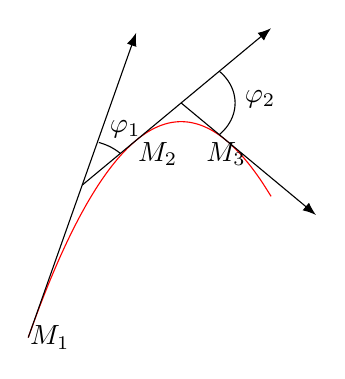
\begin{tikzpicture}[scale=1]
  \begin{axis}[clip=false,xmin=0, xmax=6,ymin=0,ymax=6, grid=none,
    xtick=\empty, ytick=\empty, axis lines=none, smooth]

    % 曲线
    \addplot[draw=red,domain=1.3:4] {-(x - 3)^2 + 4.5};

    % 导数
    % y' = -2*(x-3)

    % 切线1:y = 3.4 * x - 2.81
    \draw [-Latex] (1.3,1.61) -- (2.5,5.69);
    % 切线2:y = x + 1.75
    \draw [-Latex] (1.9,3.65) -- (2.5,4.25) -- (4,5.75);
    % 切线3:y = -x + 7.75
    \draw [-Latex] (3,4.75) -- (3.5,4.25) -- (4.5,3.25);

    % 标记
    \node [right,inner sep=0.5] at (1.3,1.61) {$M_1$};
    \node [below right,inner sep=0.5] at (2.5,4.25) {$M_2$};
    \node [below,inner sep=0.5] at (3.5,4.25) {$M_3$};

    % 倾角
    \draw [domain=45:72] plot ({1.9+0.6*cos(\x)}, {3.65+0.6*sin(\x)});
    \node [right] at (2.1,4.4) {$\varphi_1$};

    \draw [domain=-45:45] plot ({3+0.6*cos(\x)}, {4.75+0.6*sin(\x)});
    \node [right] at (3.6,4.8) {$\varphi_2$};

  \end{axis}
\end{tikzpicture}

      \subcaption{切线转过的角度$\varphi$不同}
      \label{curvature_exam1}
  \end{subfigure}
  \begin{subfigure}[t]{0.45\linewidth}
    \centering
      % 曲率,例子 2
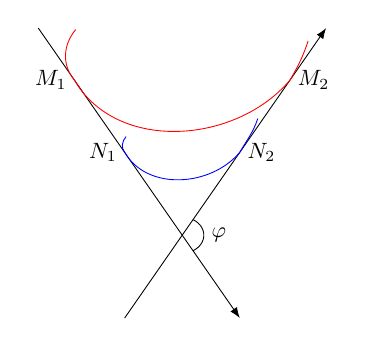
\begin{tikzpicture}[scale=0.8]
  \begin{axis}[clip=false,xmin=-3, xmax=3,ymin=-3,ymax=3, grid=none,
    xtick=\empty, ytick=\empty, axis lines=none, smooth]

    % y = 1.732 * x
    % y = -1.732 * x
    \draw [-Latex] (-0.8,-1.386) -- (2,3.464);
    \draw [-Latex] (-2,3.464) -- (0.8,-1.386);

    % -------------------------------------------------
    % 辅助线
    % \addplot[draw=blue,domain=-2.5:-0.5] {1.732 * x + 6};
    % \addplot[draw=blue,domain=0.5:2.5] {3 * x - 2};

    % 曲线 M1M2
    \draw [red] (-1.48,3.44) to [out=-130,in=130] (-1.5,2.598);
    \draw [red] (-1.5,2.598) to [out=-60,in=-130] (1.5,2.598);
    \draw [red] (1.5,2.598) to [out=60,in=-108.43] (1.75,3.25);

    % -------------------------------------------------
    % 辅助线
    % \addplot[draw=red,domain=-1.5:0] {1.732 * x + 3};
    % \addplot[draw=red,domain=0:1.5] {3 * x - 1.2};

    % 曲线 N1N2
    \draw [blue] (-0.78,1.65) to [out=-130,in=130] (-0.8,1.386);
    \draw [blue] (-0.8,1.386) to [out=-60,in=-130] (0.8,1.386);
    \draw [blue] (0.8,1.386) to [out=60,in=-108.43] (1.05,1.95);

    \node [left] at (-1.5,2.598) {$M_1$};
    \node [right] at (1.5,2.5988) {$M_2$};
    \node [left] at (-0.8,1.386) {$N_1$};
    \node [right] at (0.8,1.386) {$N_2$};

    % 倾角
    \draw [domain=-60:60] plot ({0.3*cos(\x)}, {0.3*sin(\x)});
    \node [right] at (0.3,0) {$\varphi$};

  \end{axis}
\end{tikzpicture}

      \subcaption{角度$\varphi$相同,长度不同}
      \label{curvature_exam2}
  \end{subfigure}
  \caption{曲线弧的弯曲程度}
  \label{曲线弧的弯曲程度}
\end{figure}

\subsubsection{曲率概念}
\paragraph{}
设曲线$C$是光滑的,在曲线$C$上选定一点$M_0$作为度量弧$s$的基点。设曲线上点$M$对应于弧$s$,在点$M$处切线的倾角为$\alpha$,曲线上另外一点$M'$对应于弧$s+\Delta s$,在点$M'$处切线的倾角为$\alpha+\Delta\alpha$,那么弧段$\overarc{MM'}$的长度为$|\Delta s|$,当动点从$M$移动到$M'$时切线转过的角度为$|\Delta\alpha|$。

\paragraph{}
我们用比值$\displaystyle \big|\frac{\Delta\alpha}{\Delta s}\big|$,即单位弧段上切线转过的角度的大小来表达弧段$\overarc{MM'}$的平均弯曲程度,把这比值叫做弧段$\overarc{MM'}$的\uwave{平均曲率},并记作$\overline{K}$,即

\begin{equation}
  \overline{K} = \big|\frac{\Delta\alpha}{\Delta s}\big|.
\end{equation}

\begin{figure}[H]
\centering
  % 曲率概念
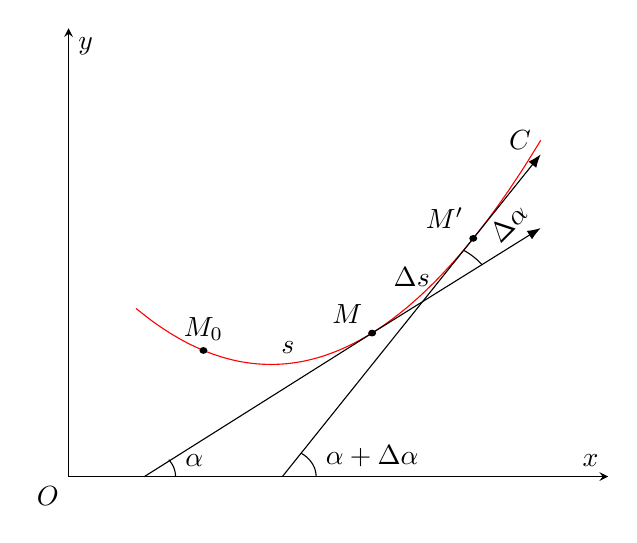
\begin{tikzpicture}[scale=1]
  \begin{axis}[clip=false,xmin=0, xmax=8,ymin=0,ymax=8, grid=none,
    xtick=\empty, ytick=\empty, axis lines=middle,
    smooth, xlabel={$x$}, ylabel={$y$}]

    % 曲线 C
    % y' = 0.5*(x-3)
    \addplot[draw=red,domain=1:7] {(x-3)^2/4 + 2};

    % 弧段
    \node [above] at (3.25,2.02) {$s$};
    \node [left] at (5.5,3.56) {$\Delta s$};

    % 切线
    % y = 0.75 * x - 0.815
    \draw [-Latex] (1.125,0) -- (4.5,2.56) -- (7,4.434);
    % y = 1.5 * x - 4.75
    \draw [-Latex] (3.17,0) -- (6,4.25) -- (7,5.75);

    % 标记
    \node [left] at (7,6) {$C$};
    \node [above] at (2,2.25) {$M_0$};
    \draw [fill] (2,2.25) circle [radius=0.05];
    \node [above left] at (4.5,2.56) {$M$};
    \draw [fill] (4.5,2.56) circle [radius=0.05];
    \node [above left] at (6,4.25) {$M'$};
    \draw [fill] (6,4.25) circle [radius=0.05];

    % 倾角
    \draw [domain=0:36.88] plot ({1.086 + 0.5*cos(\x)}, {0.5*sin(\x)});
    \node [above right] at (1.586,0) {$\alpha$};

    \draw [domain=0:56.6] plot ({3.17 + 0.5*cos(\x)}, {0.5*sin(\x)});
    \node [above right] at (3.67,0) {$\alpha + \Delta\alpha$};

    \draw [domain=36.88:56.6] plot ({5.25 + 1.1 * cos(\x)}, {3.12 + 1.1 * sin(\x)});
    \node [above right,rotate=45] at (6.4,3.9) {$\Delta\alpha$};

    % 原点
    \node [below left] at (0,0) {$O$};
  \end{axis}
\end{tikzpicture}

  \caption{曲率概念}
  \label{曲率概念}
\end{figure}

\paragraph{}
类似于从平均速度引进瞬时速度的方法,当$\Delta s \to 0$时(即$M' \to M$时),上述平均曲率的极限叫做曲线$C$在点$M$处的\uwave{曲率},记作$K$,即

\begin{equation}
  K = \lim_{\Delta s \to 0}\big|\frac{\Delta\alpha}{\Delta s}\big|.
\end{equation}

在$\displaystyle\lim_{\Delta s \to 0}\frac{\Delta\alpha}{\Delta s}=\frac{d\alpha}{ds}$存在的条件下,$K$也可以表示为
\begin{equation}
  \label{曲率的定义式}
  K = \big|\frac{d\alpha}{ds}\big|.
\end{equation}

\paragraph{}
直线的切线与本身重合,切线的倾角$\alpha$不变,曲率为$K=0$。半径为$a$的圆,其曲率为$\displaystyle K=\frac{1}{a}$。

\subsubsection{直角坐标方程的曲率计算推导}
\paragraph{}
在一般情况下,我们根据\eqref{曲率的定义式}式来导出便于实际计算曲率的公式。
\paragraph{}
设曲线的直角坐标方程是$y=f(x)$,且$f(x)$具有二阶导数(这时$f'(x)$连续,从而曲线是光滑的)。因为$\tan\alpha=y'$,所以

\begin{align}
\begin{split}
  y'' =&\; (y')' \\
      =&\; (\tan\alpha)' \quad \text{(复合函数求导法则)} \\
      =&\; \sec^2\alpha \bigcdot (\alpha)' \\
     =&\; \sec^2\alpha \bigcdot \frac{\Delta\alpha}{\Delta x},
\end{split}
\end{align}
又因为
\begin{equation}
  \tan^2\alpha + 1 = \sec^2\alpha,
\end{equation}
所以
\begin{equation}
  \frac{d\alpha}{dx} = \frac{y''}{1+\tan^2\alpha}=\frac{y''}{1+y'^2},
\end{equation}
于是
\begin{equation}
  d\alpha=\frac{y''}{1+y'^2}dx.
\end{equation}
又由\eqref{弧微分公式}知道
\begin{equation}
  ds = \sqrt{1+y'^2}dx.
\end{equation}
从而,根据曲率$K$的表达式\eqref{曲率的定义式},有
\begin{equation}
  \label{直角坐标方程的曲率计算公式}
  K = \frac{|y''|}{(1+y'^2)^{3/2}}.
\end{equation}

\subsubsection{参数方程的曲率计算推导}
\paragraph{}
设曲线由参数方程
\begin{equation}
  \left\{\begin{array}{l}
    x=\varphi(t), \\
    y=\psi(t)
  \end{array} \right.
\end{equation}
给出,则可利用由参数方程所确定的函数的求导法,求出$y'_x$及$y''_x$,代入\eqref{直角坐标方程的曲率计算公式}便得

\begin{equation}
  K=\frac{|\varphi'(t)\psi''(t)-\varphi''(t)\psi'(t)|}{[\varphi'^2(t)+\psi'^2(t)]^{3/2}}.
\end{equation}

\subsection{曲率圆与曲率半径}
\paragraph{}
设曲线$y=f(x)$在点$M(x,y)$处的曲率为$K(k\neq0)$。在点$M$处的曲线的法线上,在凹的一侧取一点$D$,使$\displaystyle|DM|=\frac{1}{K}=\rho$。以$D$为圆心,$\rho$为半径作圆,这个圆叫做曲线在点$M$处的\uwave{曲率圆},曲率圆的圆心$D$叫做曲线在点$M$处的\uwave{曲率中心},曲率圆的半径$\rho$叫做曲线在点$M$处的\uwave{曲率半径}。

\begin{figure}[H]
\centering
  % 曲率圆
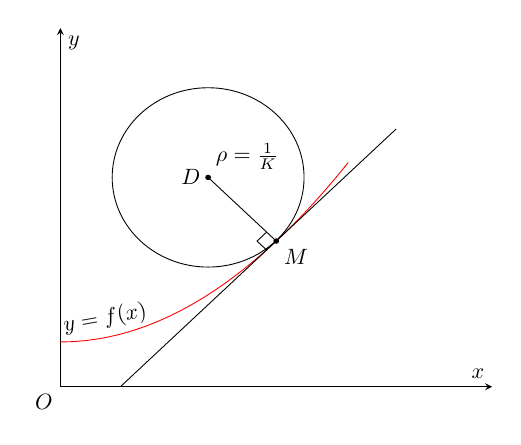
\begin{tikzpicture}[scale=0.8]
  \begin{axis}[clip=false,xmin=0, xmax=9,ymin=0,ymax=8, grid=none,
    xtick=\empty, ytick=\empty, axis lines=middle,
    smooth, xlabel={$x$}, ylabel={$y$}]

    % 曲线 y=f(x)
    % y' = 0.222 * x
    % y'' = 0.222
    \addplot[draw=red,domain=0:6] {x^2/9 + 1};

    % 弧段
    \node [above,rotate=10] at (1,1.11) {$y=f(x)$};
    \draw [fill] (4.5,3.25) circle [radius=0.05];
    \node [below right] at (4.5,3.25) {$M$};

    % 切线
    % y = x - 1.25
    \draw (1.25,0) -- (4.5,3.25) -- (7,5.75);

    % 曲率:K = 0.222 / (1+y'^2)^3/2 --> x = 4.5 --> K = 0.079
    % 半径:p = 1 / K = 12.73
    % 法线:y = -x + 7.75

    \draw [fill] (3.08,4.67) circle [radius=0.05];
    \draw (3.08,4.67) -- (4.5,3.25);
    \draw (3.08,4.67) circle [radius=2];
    \node [left] at (3.08,4.67) {$D$};
    \node [above right] at (3.08,4.67) {$\rho=\frac{1}{K}$};

    % y = -x + 7.35
    % y = x - 0.85
    \draw (4.3,3.05) -- (4.1,3.25) -- (4.3,3.45);

    % 原点
    \node [below left] at (0,0) {$O$};
  \end{axis}
\end{tikzpicture}

  \caption{曲率圆}
  \label{曲率圆}
\end{figure}

\paragraph{}
常常用曲率圆在点$M$邻近的一段圆弧来近似代替曲线弧,使问题简化。

\paragraph{}
按上述规定,曲线在点$M$处的曲率$K(k\neq0)$与曲线在点$M$处的曲率半径$\rho$有如下关系:
\begin{equation}
  \rho=\frac{1}{K}, \; K = \frac{1}{\rho}.
\end{equation}

  \section{方程的近似解}
    \subsection{方程的近似解}
\paragraph{}
求解高次代数方程或其它类型的方程的问题。求得这类方程的实根的精确值,比较困难,因此,可以寻求方程的近似解。

\begin{enumerate}
  \item 确定根的大致范围,确定一个区间$[a,b]$,使所求的根位于这区间内。这一步工作称为\uwave{根的隔离},区间$[a,b]$称为所求实根的\uwave{隔离区间}。
  \item 以根的隔离区间的端点作为根的初始近似值,逐步逼近精确值,或在精确度范围内的值。
\end{enumerate}

\subsubsection{二分法}
\paragraph{}
设$f(x)$在区间$[a,b]$上连续,$f(a)\bigcdot f(b) < 0$,且方程$f(x)=0$在$(a,b)$内仅有一个实根$\xi$,于是$[a,b]$即是这个根的一个隔离区间。

\paragraph{}
取$[a,b]$的中点$\displaystyle \xi_1 = \frac{a+b}{2}$,计算$f(\xi_1)$,然后不断缩小隔离区间的范围,不断计算中点$\xi_1$直到$f(\xi_1)=0$或在精确度之内$f(\xi_1) - 0 < \varepsilon$

\subsubsection{切线法}
\paragraph{}
用曲线弧一端的切线来代替曲线弧,从而求出方程实根的近似值。这种方法叫做\uwave{切线法}。端点的选取根据下面$4$种情况。
\begin{figure}[H]
\centering
  %------- 第1行 -------
  \begin{subfigure}[t]{0.45\linewidth}
    \centering
      % 切线法的 4 种不同情形
\begin{tikzpicture}[scale=0.8]
  \begin{axis}[clip=false,xmin=0, xmax=8,ymin=-4,ymax=4, grid=none,
    xtick=\empty, ytick=\empty, axis lines=middle,
    smooth, xlabel={$x$}, ylabel={$y$}]

    % y' = 0.15*(x-1)^0.5*x + 0.1 * (x-1)^1.5
    \addplot[draw=red,domain=1:5.5] {0.1 * (x-1)^1.5 * x - 2};

    % 实根
    \node [above] at (3.95,0) {$\xi$};

    % A
    \draw [dashed] (1,-2) -- (1,0);
    \draw [fill] (1,-2) circle [radius=0.05];
    \node [left] at (1,-2) {$A$};
    \node [above] at (1,0) {$a$};

    % B
    \draw [dashed] (5.5,3.25) -- (5.5,0);
    \draw [fill] (5.5,3.25) circle [radius=0.05];
    \node [right] at (5.5,3.25) {$B$};
    \node [below] at (5.5,0) {$b$};

    \node [below left] at (5,3.25) {$y=f(x)$};

    % 切线
    \addplot[domain=4.3:5.5] {2.7*x - 11.6};
    \node [below] at (4.3,0) {$x_1$};

    % 原点
    \node [left] at (0,0) {$O$};
  \end{axis}
\end{tikzpicture}

      \subcaption{$f(a)<0,f(b)>0$\newline$f'(x)>0,f''(x)>0$}
  \end{subfigure}
  \begin{subfigure}[t]{0.45\linewidth}
    \centering
      % 切线法的 4 种不同情形
\begin{tikzpicture}[scale=0.8]
  \begin{axis}[clip=false,xmin=0, xmax=8,ymin=-4,ymax=4, grid=none,
    xtick=\empty, ytick=\empty, axis lines=middle,
    smooth, xlabel={$x$}, ylabel={$y$}]

    % y' = -20*(x+1)^-2
    \addplot[draw=red,domain=1.5:6] {20/(x+1) - 5};

    % 实根
    \node [above] at (3,0) {$\xi$};

    % A
    \draw [dashed] (1.5,3) -- (1.5,0);
    \draw [fill] (1.5,3) circle [radius=0.05];
    \node [left] at (1.5,3) {$A$};
    \node [below] at (1.5,0) {$a$};

    \node [below right] at (1.8,3) {$y=f(x)$};

    % 切线
    \addplot[domain=1.5:2.44] {-3.2*x + 7.8};
    \node [below] at (2.44,0) {$x_1$};

    % B
    \draw [dashed] (6,-2.14) -- (6,0);
    \draw [fill] (6,-2.14) circle [radius=0.05];
    \node [right] at (6,-2.14) {$B$};
    \node [above] at (6,0) {$b$};

    % 原点
    \node [left] at (0,0) {$O$};
  \end{axis}
\end{tikzpicture}

      \subcaption{$f(a)>0,f(b)<0$\newline$f'(x)<0,f''(x)>0$}
  \end{subfigure}
  %------- 第2行 -------
  \begin{subfigure}[t]{0.45\linewidth}
    \centering
      % 切线法的 4 种不同情形
\begin{tikzpicture}[scale=0.8]
  \begin{axis}[clip=false,xmin=0, xmax=8,ymin=-4,ymax=4, grid=none,
    xtick=\empty, ytick=\empty, axis lines=middle,
    smooth, xlabel={$x$}, ylabel={$y$}]

    % y' = 3/x
    \addplot[draw=red,domain=1.5:6] {3*ln(x) - 3.5};

    % 实根
    \node [below] at (3.23,0) {$\xi$};

    % A
    \draw [dashed] (1.5,-2.28) -- (1.5,0);
    \draw [fill] (1.5,-2.28) circle [radius=0.05];
    \node [left] at (1.5,-2.28) {$A$};
    \node [above] at (1.5,0) {$a$};

    % 切线
    \addplot[domain=1.5:2.64] {2*x - 5.28};
    \node [above] at (2.64,0) {$x_1$};

    % B
    \draw [dashed] (6,1.88) -- (6,0);
    \draw [fill] (6,1.88) circle [radius=0.05];
    \node [right] at (6,1.88) {$B$};
    \node [below] at (6,0) {$b$};

    \node [below left] at (5,1.88) {$y=f(x)$};

    % 原点
    \node [left] at (0,0) {$O$};
  \end{axis}
\end{tikzpicture}

      \subcaption{$f(a)<0,f(b)>0$\newline$f'(x)>0,f''(x)<0$}
  \end{subfigure}
  \begin{subfigure}[t]{0.45\linewidth}
    \centering
      % 切线法的 4 种不同情形
\begin{tikzpicture}[scale=0.8]
  \begin{axis}[clip=false,xmin=0, xmax=8,ymin=-4,ymax=4, grid=none,
    xtick=\empty, ytick=\empty, axis lines=middle,
    smooth, xlabel={$x$}, ylabel={$y$}]

    % -0.6*(x-1)^0.8
    \addplot[draw=red,domain=1:6] {-0.33*(x-1)^1.8+2.5};

    % 实根
    \node [below left] at (4.248,0) {$\xi$};

    % A
    \draw [dashed] (1,2.5) -- (1,0);
    \draw [fill] (1,2.5) circle [radius=0.05];
    \node [left] at (1,2.5) {$A$};
    \node [below] at (1,0) {$a$};

    \node [below right] at (2.5,2.5) {$y=f(x)$};

    % B
    \draw [dashed] (6,-3.48) -- (6,0);
    \draw [fill] (6,-3.48) circle [radius=0.05];
    \node [right] at (6,-3.48) {$B$};
    \node [above] at (6,0) {$b$};

    % 切线
    \addplot[domain=4.41:6] {-2.17*x + 9.57};
    \node [above] at (4.41,0) {$x_1$};

    % 原点
    \node [left] at (0,0) {$O$};
  \end{axis}
\end{tikzpicture}

      \subcaption{$f(a)>0,f(b)<0$\newline$f'(x)<0,f''(x)<0$}
  \end{subfigure}

  \caption{切线的$4$种不同情形}
  \label{切线的4种不同情形}
\end{figure}

\paragraph{}
假设选取端点为$a$的情形,令$x_0 = a$,在端点$(x_0,f(x_0))$作切线,这切线的方程为
\begin{equation*}
  y - f(x_0) = f'(x_0)(x-x_0)
\end{equation*}
令$y=0$,可以解出$x_1$为
\begin{equation*}
  x_1 = x_0 - \frac{f(x_0)}{f'(x_0)}
\end{equation*}

\paragraph{}
然后继续在点$(x_1,f(x_1))$作切线,直到逼近$\xi$,一般的,在点$(x_{n-1},f(x_{n-1}))$作切线,得根的近似值
\begin{equation}
  x_n = x_{n-1} - \frac{f(x_{n-1})}{f'(x_{n-1})}.
\end{equation}

\end{document}
